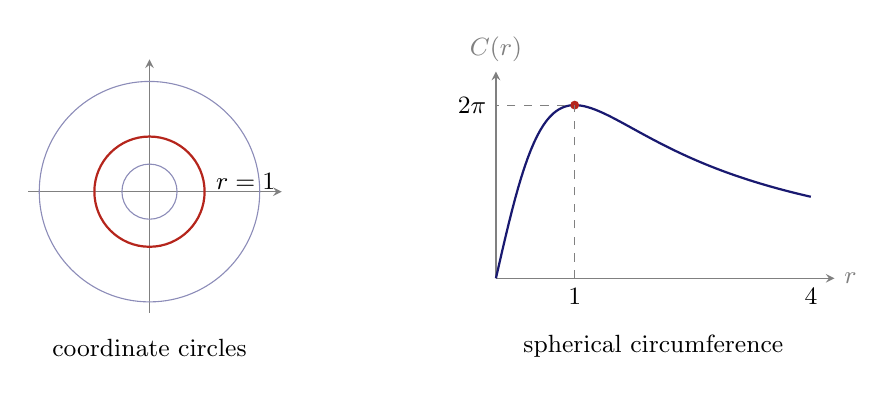
\begin{tikzpicture}[x=1cm,y=1cm,font=\small,>=stealth]
\begin{scope}[x=.7cm,y=.7cm]
\draw[gray,->] (-2.2,0)--(2.4,0);
\draw[gray,->] (0,-2.2)--(0,2.4);
\draw[MidnightBlue!50] (0,0) circle (.5);
\draw[BrickRed,thick] (0,0) circle (1);
\draw[MidnightBlue!50] (0,0) circle (2);
\node[right] at (1.03,.18) {$r=1$};
\node[below] at (0,-2.5) {coordinate circles};
\end{scope}
\begin{scope}[shift={(4.4,-1.1)},x=1cm,y=.35cm]
\draw[gray,->] (0,0)--(4.3,0) node[right] {$r$};
\draw[gray,->] (0,0)--(0,7.5) node[above] {$C(r)$};
\draw[MidnightBlue,thick,domain=0:4,samples=100] plot (\x,{4*pi*\x/(1+\x*\x)});
\fill[BrickRed] (1,{2*pi}) circle (1.6pt);
\draw[gray,dashed] (1,0)--(1,{2*pi})--(0,{2*pi});
\node[left] at (0,{2*pi}) {$2\pi$};
\node[below] at (1,0) {$1$};
\node[below] at (4,0) {$4$};
\node[below] at (2,-1.7) {spherical circumference};
\end{scope}
\end{tikzpicture}
